\documentclass{sigchi}
\usepackage{xspace}
\usepackage{fancyvrb}
\usepackage{inconsolata}
\usepackage{xcolor}

\definecolor{kvdclr}{rgb}{0.3,0.0,0.8}
\DefineVerbatimEnvironment{thegamma}{Verbatim}{fontfamily=zi4,numbers=left,xleftmargin=6mm,fontsize=\small,commandchars=\\\{\}}
%\newcommand{\kvd}[1]{\textcolor{kvdclr}{#1}}
\newcommand{\kvd}[1]{\textbf{#1}}
\newcommand{\ikvd}[1]{{\fontfamily{zi4}\selectfont #1}}
\newcommand{\tg}{The Gamma\xspace}

% Use this section to set the ACM copyright statement (e.g. for
% preprints).  Consult the conference website for the camera-ready
% copyright statement.

% Copyright
\CopyrightYear{2020}
%\setcopyright{acmcopyright}
\setcopyright{acmlicensed}
%\setcopyright{rightsretained}
%\setcopyright{usgov}
%\setcopyright{usgovmixed}
%\setcopyright{cagov}
%\setcopyright{cagovmixed}
% DOI
\doi{https://doi.org/10.1145/3313831.XXXXXXX}
% ISBN
\isbn{978-1-4503-6708-0/20/04}
%Conference
\conferenceinfo{UIST'20,}{October  20--23, 2020, Minneapolis, MN, USA}
%Price
\acmPrice{\$15.00}

% Use this command to override the default ACM copyright statement
% (e.g. for preprints).  Consult the conference website for the
% camera-ready copyright statement.

%% HOW TO OVERRIDE THE DEFAULT COPYRIGHT STRIP --
%% Please note you need to make sure the copy for your specific
%% license is used here!
% \toappear{
% Permission to make digital or hard copies of all or part of this work
% for personal or classroom use is granted without fee provided that
% copies are not made or distributed for profit or commercial advantage
% and that copies bear this notice and the full citation on the first
% page. Copyrights for components of this work owned by others than ACM
% must be honored. Abstracting with credit is permitted. To copy
% otherwise, or republish, to post on servers or to redistribute to
% lists, requires prior specific permission and/or a fee. Request
% permissions from \href{mailto:Permissions@acm.org}{Permissions@acm.org}. \\
% \emph{UIST '20},  October 20--23, 2020, Minneapolis, MN, USA \\
% ACM xxx-x-xxxx-xxxx-x/xx/xx\ldots \$15.00 \\
% DOI: \url{http://dx.doi.org/xx.xxxx/xxxxxxx.xxxxxxx}
% }

% Arabic page numbers for submission.  Remove this line to eliminate
% page numbers for the camera ready copy
% \pagenumbering{arabic}

% Load basic packages
\usepackage{balance}       % to better equalize the last page
\usepackage{graphics}      % for EPS, load graphicx instead
\usepackage[T1]{fontenc}   % for umlauts and other diaeresis
\usepackage{txfonts}
\usepackage{mathptmx}
\usepackage[pdflang={en-US},pdftex]{hyperref}
\usepackage{color}
\usepackage{booktabs}
\usepackage{textcomp}

% Some optional stuff you might like/need.
\usepackage{microtype}        % Improved Tracking and Kerning
% \usepackage[all]{hypcap}    % Fixes bug in hyperref caption linking
\usepackage{ccicons}          % Cite your images correctly!
% \usepackage[utf8]{inputenc} % for a UTF8 editor only

% If you want to use todo notes, marginpars etc. during creation of
% your draft document, you have to enable the "chi_draft" option for
% the document class. To do this, change the very first line to:
% "\documentclass[chi_draft]{sigchi}". You can then place todo notes
% by using the "\todo{...}"  command. Make sure to disable the draft
% option again before submitting your final document.
\usepackage{todonotes}

% Paper metadata (use plain text, for PDF inclusion and later
% re-using, if desired).  Use \emtpyauthor when submitting for review
% so you remain anonymous.
\def\plaintitle{The Gamma: Data Exploration through Iterative Prompting}
\def\plainauthor{First Author, Second Author, Third Author,
  Fourth Author, Fifth Author, Sixth Author}
\def\emptyauthor{}
\def\plainkeywords{Data exploration; End-user programming; Data journalism; Programming languages; Type providers}
\def\plaingeneralterms{Documentation, Standardization}

% llt: Define a global style for URLs, rather that the default one
\makeatletter
\def\url@leostyle{%
  \@ifundefined{selectfont}{
    \def\UrlFont{\sf}
  }{
    \def\UrlFont{\small\bf\ttfamily}
  }}
\makeatother
\urlstyle{leo}

% To make various LaTeX processors do the right thing with page size.
\def\pprw{8.5in}
\def\pprh{11in}
\special{papersize=\pprw,\pprh}
\setlength{\paperwidth}{\pprw}
\setlength{\paperheight}{\pprh}
\setlength{\pdfpagewidth}{\pprw}
\setlength{\pdfpageheight}{\pprh}

% Make sure hyperref comes last of your loaded packages, to give it a
% fighting chance of not being over-written, since its job is to
% redefine many LaTeX commands.
\definecolor{linkColor}{RGB}{6,125,233}
\hypersetup{%
  pdftitle={\plaintitle},
% Use \plainauthor for final version.
%  pdfauthor={\plainauthor},
  pdfauthor={\emptyauthor},
  pdfkeywords={\plainkeywords},
  pdfdisplaydoctitle=true, % For Accessibility
  bookmarksnumbered,
  pdfstartview={FitH},
  colorlinks,
  citecolor=black,
  filecolor=black,
  linkcolor=black,
  urlcolor=linkColor,
  breaklinks=true,
  hypertexnames=false
}

% create a shortcut to typeset table headings
% \newcommand\tabhead[1]{\small\textbf{#1}}

% End of preamble. Here it comes the document.
\begin{document}

\title{\plaintitle}

\numberofauthors{3}
\author{%
  \alignauthor{Leave Authors Anonymous\\
    \affaddr{for Submission}\\
    \affaddr{City, Country}\\
    \email{e-mail address}}\\
  \alignauthor{Leave Authors Anonymous\\
    \affaddr{for Submission}\\
    \affaddr{City, Country}\\
    \email{e-mail address}}\\
  \alignauthor{Leave Authors Anonymous\\
    \affaddr{for Submission}\\
    \affaddr{City, Country}\\
    \email{e-mail address}}\\
}

\maketitle

\begin{abstract}
Governments, non-profit organizations and citizen initiatives publish increasing amounts of
data, but extracting insights from such data and presenting them to the public is hard.
First, data comes in a variety of formats that each requires a different tool. Second, many
data exploration tools do not reveal how a result was obtained, making it difficult to reproduce
the results and check how they were obtained.
%
We contribute The Gamma, a novel data exploration environment for non-experts. The Gamma is based
on a single interaction principle and using it results in transparent and reproducible scripts.
This allows transfer of knowledge from one data source to another and
learning from previously created data analyses. We evaluate the usability and learnability of
The Gamma through a user study on non-technical employees of a research institute.
%
We argue that the our approach allows journalists and the public to benefit from the rise
of open data, by making data exploration easier, more transparent and more reproducible.
\end{abstract}


% ACM Classfication
%
% \begin{CCSXML}
% <ccs2012>
% <concept>
% <concept_id>10003120.10003121</concept_id>
% <concept_desc>Human-centered computing~Human computer interaction (HCI)</concept_desc>
% <concept_significance>500</concept_significance>
% </concept>
% <concept>
% <concept_id>10003120.10003121.10003125.10011752</concept_id>
% <concept_desc>Human-centered computing~Haptic devices</concept_desc>
% <concept_significance>300</concept_significance>
% </concept>
% <concept>
% <concept_id>10003120.10003121.10003122.10003334</concept_id>
% <concept_desc>Human-centered computing~User studies</concept_desc>
% <concept_significance>100</concept_significance>
% </concept>
% </ccs2012>
% \end{CCSXML}
%
% \ccsdesc[500]{Human-centered computing~Human computer interaction (HCI)}
% \ccsdesc[300]{Human-centered computing~Haptic devices}
% \ccsdesc[100]{Human-centered computing~User studies}

% Author Keywords
\keywords{\plainkeywords}

% Print the classficiation codes
% \printccsdesc
% Please use the 2012 Classifiers and see this link to embed them in the text: \url{https://dl.acm.org/ccs/ccs_flat.cfm}

\begin{figure}
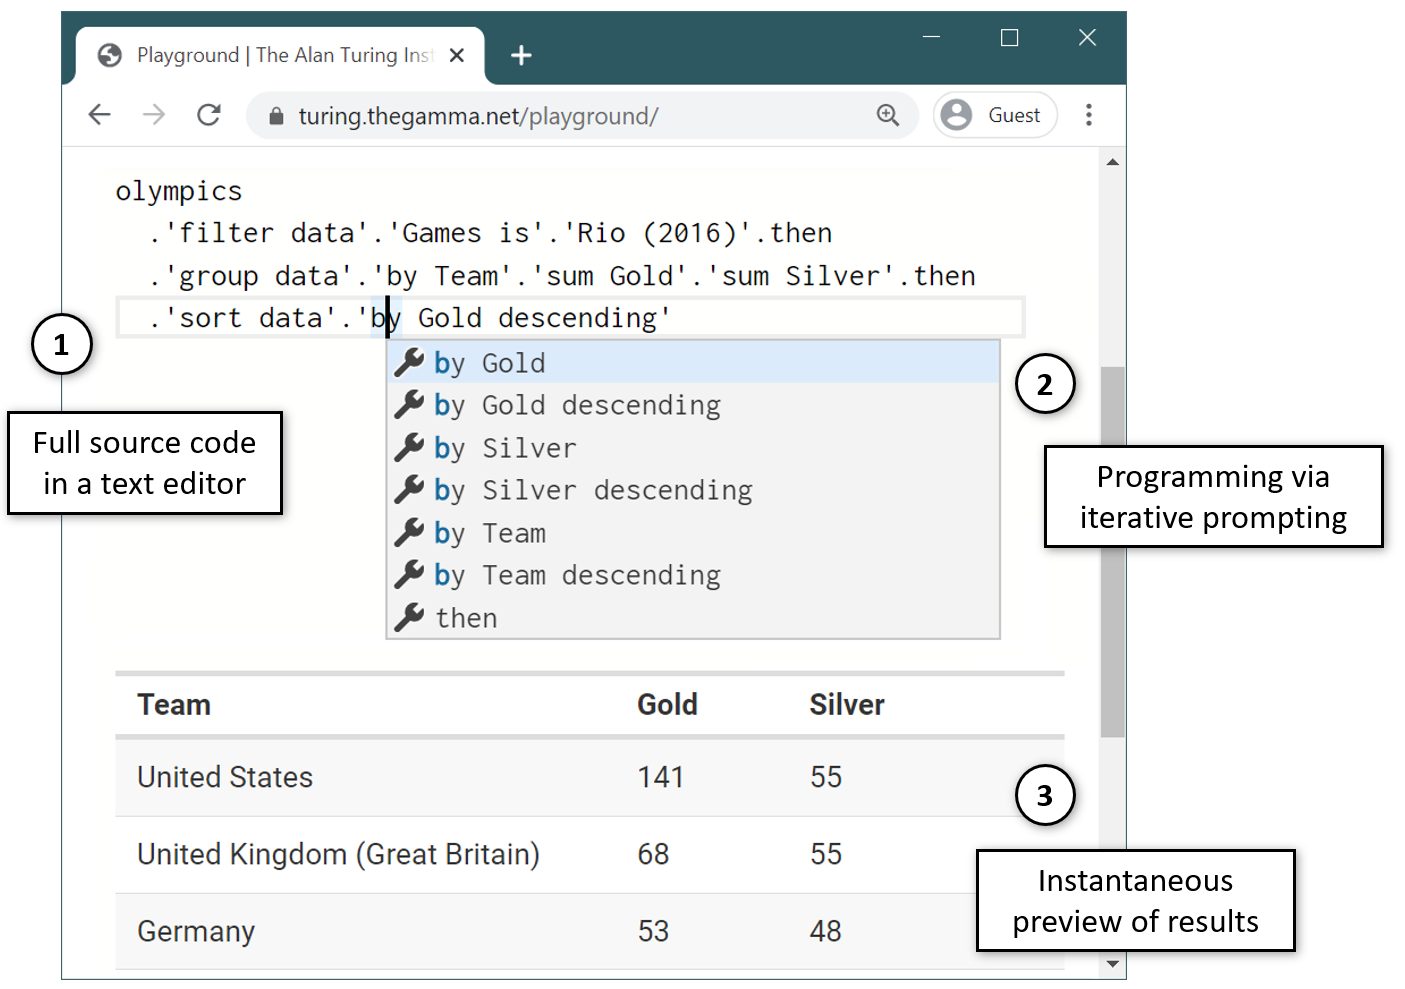
\includegraphics[width=1\columnwidth]{figures/thegamma-annot}
\caption{Teams with the greatest number of gold medals from Rio 2016
Olympics with a reproducible The Gamma script (1), an auto-complete prompt offering ways
of sorting the data (2) and instant preview (3).}
\label{fig:thegamma}
\vspace{-0.5em}
\end{figure}


\section{Introduction}
Data science has more capabilities to help us understand the world than ever before, yet at the
same time post-truth politics and increasing public distrust in statistics makes data-driven insights
increasingly less relevant in public discourse~\cite{howstatslost}. This should perhaps not be a surpirse.
Journalists can access increasing amounts of data, but producing engaging and transparent data-driven
reports that are easy to interpret is expensive and requires expert programming skills \cite{ddj}.

The design of a data exploration tool for journalists poses a unique mix of challenges. First, the
tool needs to be easy to learn for end-users working under tight deadlines. Second, it needs to
support a wide range of data sources in a way where the expertise gained when working with one data
source is relevant for other data sources. Third, the resulting data-driven insights need to be
transparent, allowing the readers to verify the claims and learn how to reproduce the work.

We present The Gamma, a text-based data exploration environment for non-experts. The Gamma
is based on a single interaction principle, which provides uniform
access to a range of data sources including data tables, graph databases and data cubes.
An anlysis created in The Gamma is a transparent script that can be followed to reproduce the
result from scratch. This allows learning from existing analyses and encourages readers
to engage with the results. Our key contributions are:

\begin{itemize}
\item We identify the design requirements for a data exploration tool for journalists
  (Section~\ref{sec:motivation}) and follow those to build a novel programming environment
  The Gamma (Section~\ref{sec:overview}).

\item We introduce \emph{iterative prompting} (Section~\ref{sec:design}),
  an interaction design principle that can be used to complete a variety of programming
  tasks in a uniform way that allows transfer of knowledge between different tasks.

\item We show how to use the iterative prompting principle for querying of distinct data
  sources including data tables, graph databases and data cubes (Section~\ref{sec:implementation}).

\item We discuss a number of case studies (Section~\ref{sec:cases}) and
  conduct a user study to evaluate the usability of The Gamma and the extent to which users can,
  (i) learn from examples and (ii)~transfer knowledge between tasks (Section~\ref{sec:study}).
\end{itemize}

The Gamma is available as open-source at \href{http://thegamma.net}{\small\bf\ttfamily thegamma.net}.

\section{Related work}

\textbf{Visual tools.}

\textbf{Programming tools.}
Notebooks

\textbf{Journalism.}
Idyll \cite{idyll}

\textbf{Type providers.}
PL work

\newpage
~
\newpage

\begin{figure}
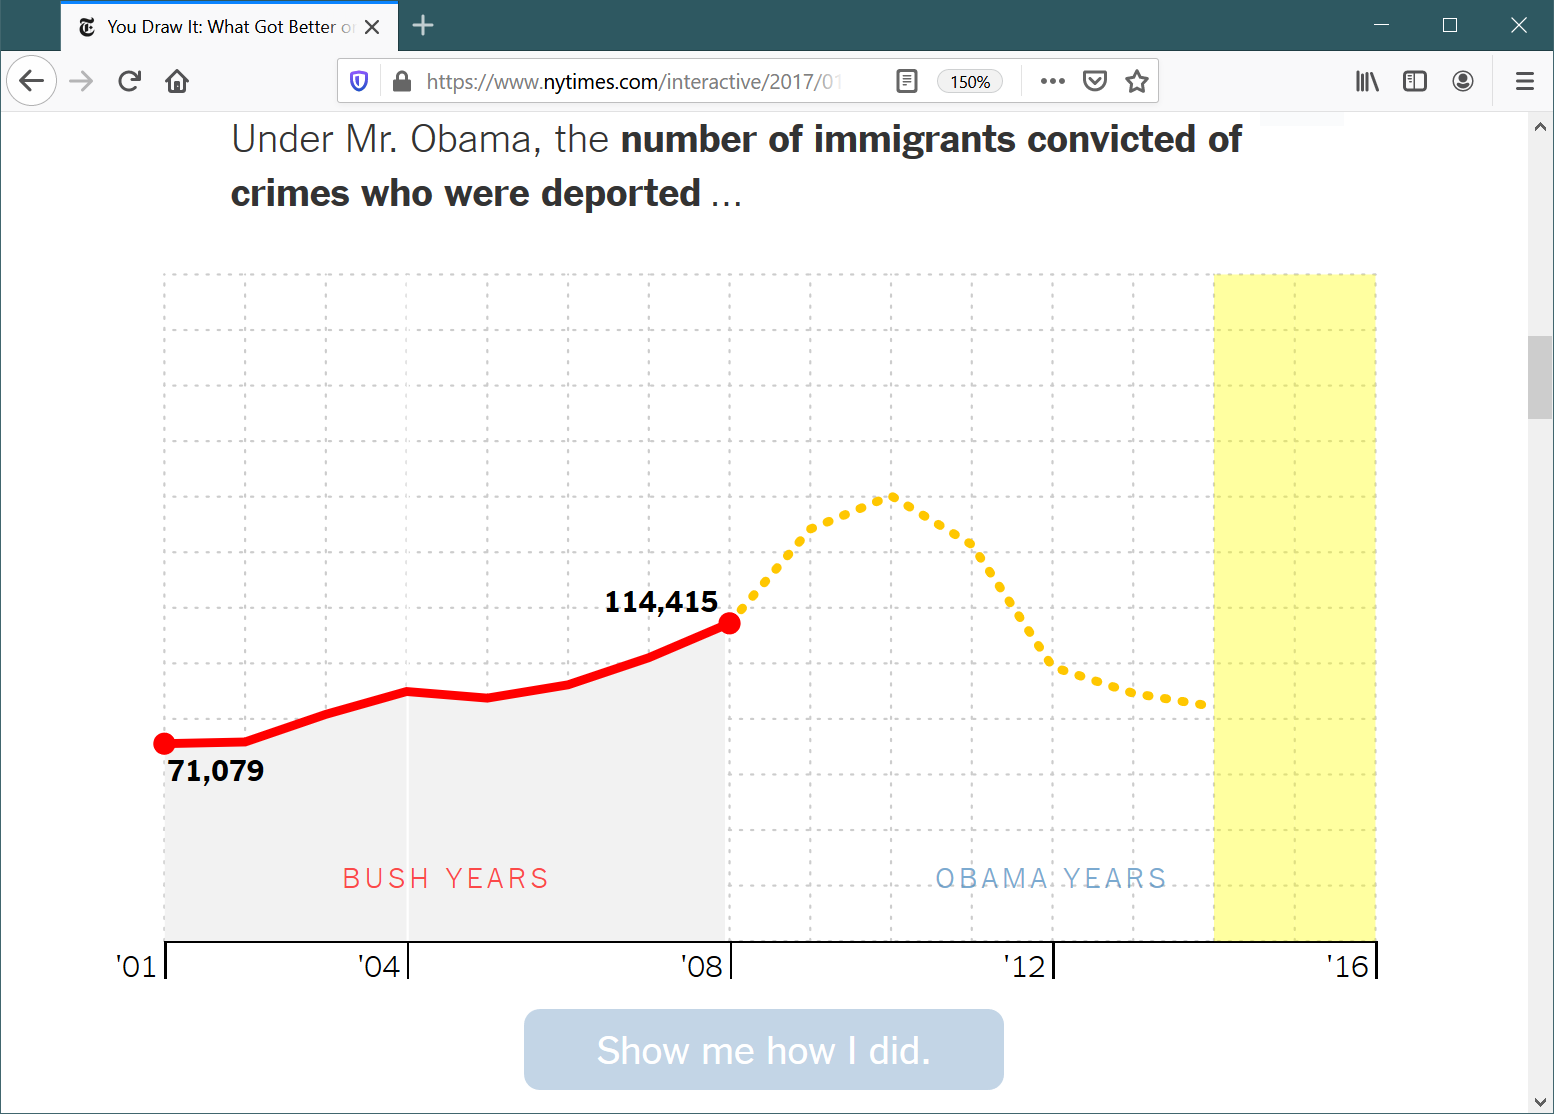
\includegraphics[width=1\columnwidth]{figures/nyt}
\caption{New York Times article on Obama's legacy \cite{youdraw}. The article asks the reader to make a guess
(engagement), but only lists ``Immigration and Customs Enforcement'' as a source of data.}
\label{fig:nyt}
\end{figure}

\section{Background and design goals}
\label{sec:motivation}

The Gamma aims to adapt the recent innovations in programming language research, especially the
work on type providers, into a form where it could be used in practice by journalists and other
non-expert interested in data exploration. We start with a careful consideration of our target
application domain, i.e.~data analyses produced by journalists and citizen data scientists that
are published online. We look at both practical requirements for such programming environment
and requirements arising from our focus on journalism. This analysis is based on the author's
experience of collaborating with journalists\footnote{Citations removed to preserve anonymity.},
review of literature on data journalism, e.g.~\cite{ddj,edcj17,edcj18} and more general trends in
journalism.

\subsection{Open Journalism}
Journalism continually develops and responds to the many challenges it faces \cite{future}.
Two recent challenges are relevant to our work. The first is building trust in media.
One way of establishing trust in the age of fake news is to be more transparent about editorial
decisions, process and original sources. Many journalists believe that opening up the process
shows the quality and trustworthiness of their work~\cite{transparency}.
The second challenge is reader engagement. To develop a relationship with readers, journalists are
increasingly looking for meaningful ways of engagement. This includes reader comments, involvement
of citizen journalists \cite{comments,citizen} and the development of new interactive formats
\cite{youdraw}. To address the above challenges, a tool for data exploration should satisfy the
following three requirements.

\paragraph{Trust Through Transparency}
To support trustworthiness, data analyses should be transparent. The reader should be able to
determine what is the source of analysed data and how has the data been transformed. As much as
possible, these capabilities should also be accessible to non-expert readers.

\paragraph{Reproducibility for Fact Checking}
It should be possible to re-run the analysis to verify that it produces the presented results.
However, running an opaque script is not enough. A reader should be able to recreate the analysis
by following the necessary steps from the original data source to the end result.

\paragraph{Encouraging Meaningful Engagement}
The tool should support a mechanism through which readers can engage in a meaningful discussion.
For example, it should allow modifying of parameters of a data visualization in order to show
how different choices affect the final result.

\begin{figure}
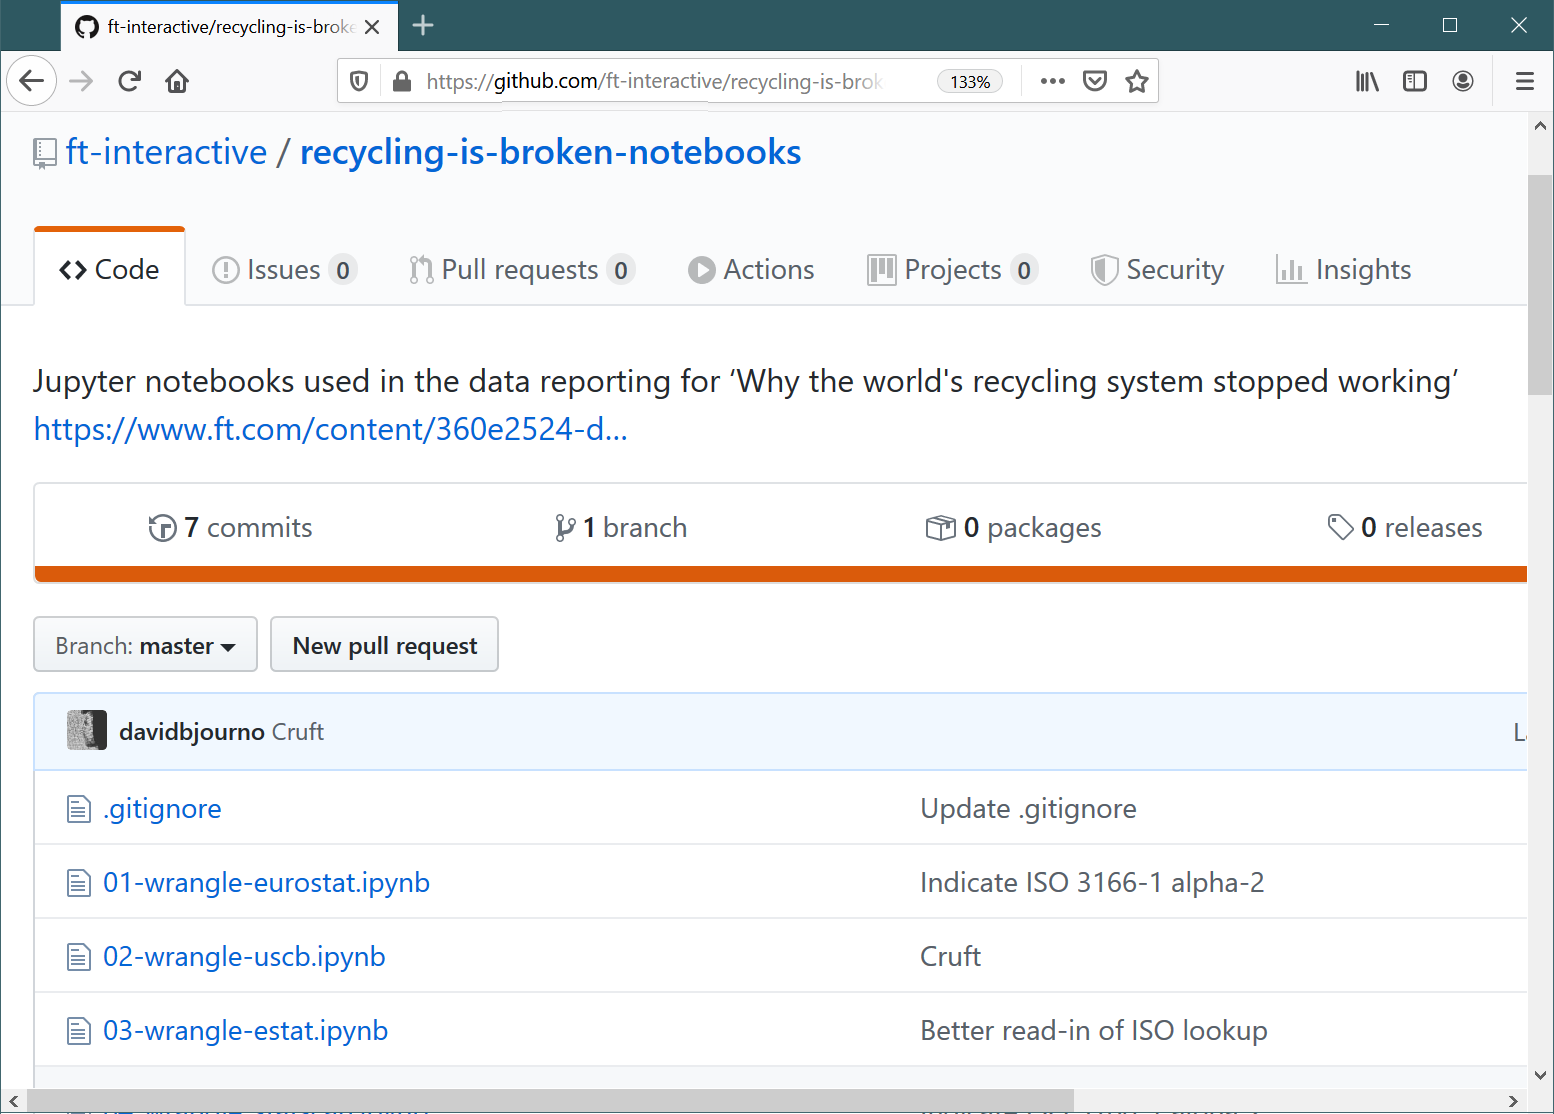
\includegraphics[width=1\columnwidth]{figures/ft}
\caption{Financial Times analysis of recyclable waste. Full source is provided as Jupyter Notebooks
on GitHub \cite{ftnotebooks}, but re-running the analysis is difficult, even for an expert.}
\label{fig:ft}
\end{figure}

\subsection{End-user Data Exploration}
Our aim is to make programmatic data exploration accessible to journalists, but we want to keep
the desirable properties of text-based programming. In particular, source code of a data
exploration should provide a full reproducible record of how the data analysis has been done.
As end-users, journalists have a number of interesting characteristics. They work under tight
deadline and data exploration is only a complementary skill. They also need to work with a wide
range of data sources, including big data tables (e.g.~Iraq War documents leak) or graph
databases (e.g.~Panama Papers). This leads to a number of practical requirements on the programming
environment.

\paragraph{Conceptual Simplicity}
We target end-users who cannot dedicate much time to learning about a tool prior
to using it. Consequently, using the tool should require understanding of only a small number
of concepts. Once the user understand a small number of concepts, they should be able to complete
basic data exploration tasks.

\paragraph{Uniformity across Data Sources}
The users should be able to navigate through large databases, query relational databases and
query graph databases through the same mechanism. Ideally, expertise gained with one data source
should also be transferable to working with another data source.

\paragraph{Learning without Experts}
Sarkar \cite{learning} reports that users learn how to use Excel either by talking to experts,
or by seeing a feature in a spreadsheet received from a colleague. In our circumstances, experts
are unlikely to be available, so the tool should support learning from examples. When looking at
a work done and published by another person, the user needs to see (and be able to understand)
how a task was completed.

\newpage
~
\newpage


\section{Overview}
\label{sec:overview}

\tg is a text-based programming environment that allows non-experts create simple data exploration
scripts using a single interaction principle -- choosing an item from an auto-complete list.
It supports a range of data sources including tabular data, graph data and data cubes.

\subsection{Querying Travel Expenses}
To introduce \tg, we walk through a simple problem that a local journalist might want to solve.
The UK government publishes travel expense claims by members of the House of Lords. A journalist
wants to find out which of the members representing the Kent county spend the most on travel.
The following shows a subset of the data:\footnote{ \url{https://www.parliament.uk/mps-lords-and-offices/members-allowances/house-of-lords/holallowances/} }

\begin{thegamma}
\textbf{Name, County, Days Attended, Days Away, Travel Costs}
Lord Adonis, London, 8, 0, 504
Baroness Afshar, Yorkshire, 2, 0, 0
Lord Alderdice, Oxfordshire, 3, 0, 114
Lord Alli, London, 5, 0, 0
Baroness Amos, London, 3, 0, 0
\end{thegamma}

After the analyst imports the CSV file (through a web interface), the environment is initialized
with code that refers to the imported variable \ikvd{expenses}. The analyst then types `.' (dot):

\begin{thegamma}
expenses.
\end{thegamma}
\vspace{-0.4em}\qquad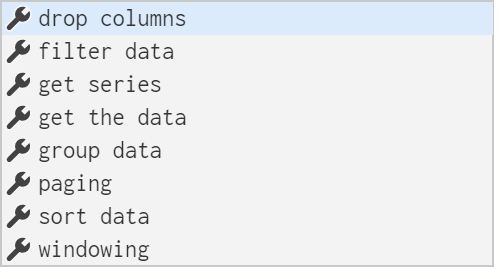
\includegraphics[width=0.5\columnwidth]{figures/lords1}

The type provider for tabular data allows analysts to construct simple queries. It first offers
a list of operations that the analyst might want to perform such as grouping, filtering and sorting.
To find members of the House of Lords from Kent, the analyst chooses \ikvd{filter data},
types `.' and then chooses \ikvd{County is} from the offered list, types `.' and starts
typing Kent:

\begin{thegamma}
expenses
  .'filter data'.'County is'.Ke
\end{thegamma}
\vspace{-0.4em}\qquad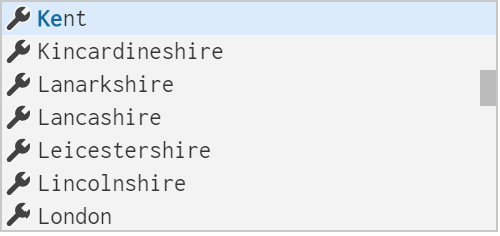
\includegraphics[width=0.5\columnwidth]{figures/lords2}

The completion list is generated from the values in the \ikvd{County} column of the dataset.
After selecting \ikvd{Kent}, the live preview is updated to only show records according to the
specified filter:

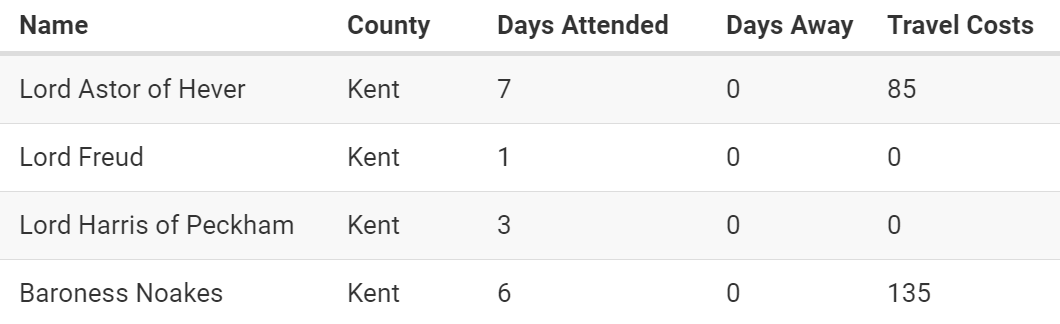
\includegraphics[width=1\columnwidth]{figures/lords3}

To finish specifying filtering conditions, the analyst chooses \ikvd{then} and is offered the
same list of querying operations as in the first step. To sort House of Lords members by their
travel costs, she now chooses \ikvd{sort data} and types `.' (dot):

\begin{thegamma}
expenses
  .'filter data'.'County is'.Kent.then
  .'sort data'.
\end{thegamma}
\qquad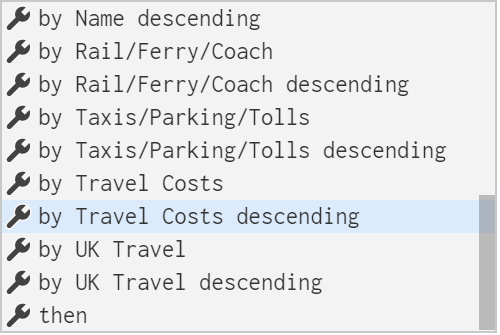
\includegraphics[width=0.5\columnwidth]{figures/lords4}

The auto-complete offers a list of columns that can be used for sorting, each with ascending
(default) and descending order option. After choosing one or more sort keys, the analyst selects
the \ikvd{then} member and is, again, offered the list of querying operations. They use
\ikvd{paging} to get top 5 records and \ikvd{get series} to obtain a data series with just
the House of Lords member name and their travel expenses.

\begin{thegamma}
expenses
  .'filter data'.'County is'.Kent.then
  .'sort data'.'by Travel Costs descending'.then
  .paging.take(5)
  .'get series'.'with key Name'.'and value Travel Costs'
\end{thegamma}

When the code evaluates to a data series with a categorical (textual) key and a numerical value,
\tg switches from displaying the result as a table to a column chart:

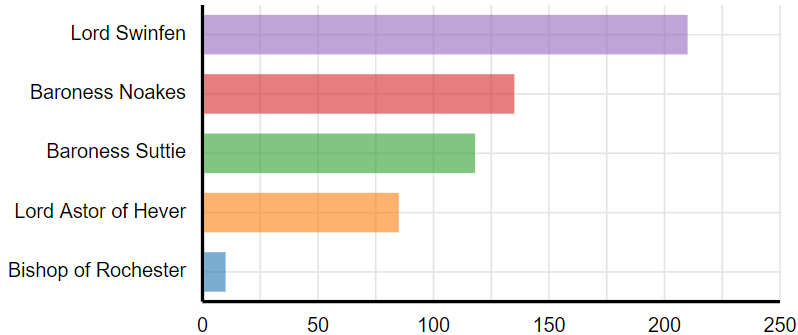
\includegraphics[width=1\columnwidth]{figures/lords5}

\subsection{Querying via Iterative Prompting}
The



\newpage


\section{Design}
\label{sec:design}


interaction = iterative prompting
how is this different from just auto-complete?

trace = for transparency and learning

One important observation from the above list is that our tool should be accessible to non-expert
users such as readers and non-technical journalists, while providing extra capabilities for more
technical users. It should be easy to use if one just wants to modify existing code and should
encourage experimentation. Considering these challenges, we identify the following technical
design principles. todo{There must be papers on learning programming that can be referenced
here.}

\paragraph{B1. Learning from examples and by experimentation.} We should support two ways of learning.
Users of tools such as spreadsheets
often learn by looking at existing problem solutions todo{Advait's PPIG}. Our design should allow
this by making it possible to inspect and retrace steps used while solving a problem in an existing
application. Another principle of spreadsheets that we want to keep is the ability to experiment
and see results immediately. Our design should allow users to try invoking an operation or modifying
a parameter and quickly see if this leads to the desired results.

\paragraph{B2. Choice over construction.} To minimize the amount of information that users have to
learn and remember, our system should work in a way that allows constructing programs by
choosing from options that can reasonably appear in a current context, rather than requiring
users to recall particular syntax or exact identifier name.
todo{recognition over recall?}

\paragraph{B3. Make simple things easy and complex things possible.} Some users of the system may, over time, become advanced users
and the system should support those. In other words, the upper bound on what can be achieved
should be well above the most common use cases. At the same time, the complex features that power users might
need should not affect the most elementary uses of the system and should remain completely hidden
until needed. In other words, the lower bound on what one needs to know to use the system for basic
tasks should be as low as possible. todo{I think I got this idea of "boundaries" on what
is possible from some paper, but cannot recall which...}

\paragraph{B4. Visibility of state.} To support transparency, the system should make its entire state
transparent -- when reviewing a data analysis, all parameters should be immediately visible and the
user should not need to, e.g.~navigate through complex user interface to find them.

\section{Implementation}
\label{sec:implementation}

\subsection{Language}

\subsection{Type providers}

\section{Use cases}
\label{sec:cases}

\section{User study}
\label{sec:study}

this is between-user user study

FIRST: How one area transfers to another?


DEMO: WorldBank
explain everything

DISPLAY: Public order and safety, Defence
\begin{verbatim}
expenditure.byService.'Public order and safety'.inTermsOf.GDP
expenditure.byService.Defence.inTermsOf.GDP
\end{verbatim}

DEMO: Graph DB
explain everything

\begin{verbatim}
drWho.Character.Doctor.'ENEMY_OF'.'[any]'
  .'APPEARED_IN'.'[any]'.'explore_properties'.explore
  .'group data'.'by 1-name'.'count distinct 2-title'
\end{verbatim}

DISPLAY: Who has larges travel expenses?
(and in London only?)

\begin{verbatim}
lords.'sort data'.'by Travel Costs descending'

lords
  .'filter data'.'County is'.London.then
  .'sort data'.'by Travel Costs descending'
\end{verbatim}

SECOND: No experts are needed

DEMO: explain how live preview works, explain how '.' works,
explain how newlines and indentation work

DISPLAY 'CO2 emissions (metric tons per capita)'

\begin{verbatim}
worldbank.byCountry.'United Kingdom'
  .'Economy & Growth'.'GDP per capita (current US$)'

worldbank.byCountry.Germany
  .'Economy & Growth'.'GDP per capita (current US$)'

worldbank.byCountry.'Czech Republic'
  .'Economy & Growth'.'GDP per capita (current US$)'
\end{verbatim}


DISPLAY: Top athletes from London

\begin{verbatim}
olympics
  .'group data'.'by Team'.'sum Gold'.then
  .'sort data'.'by Gold descending'.then
  .paging.take(5)
  .'get series'.'with key Team'.'and value Gold'
\end{verbatim}


THIRD: 'then'

DEMO: Show worldbank
GIVE: Commented source code using 'olympics'
DISPLAY: Top athletes from London (think-aloud)

QUESTIONS

1) Did I tell you enough in the introduction to get started?

Say we want to provide educational materials for journalists
(with limited budgets), what would be the most important?

2) Video or just code samples?

We'll have more data sources than we can write tutorials for

3) Do we just teach them how the environment works?

4) What do we need to teach about a data source?


\section{Discussion}

\subsection{Study limitations}
exploratory in nature so we do not make any quantitative claims about effects

not comparing against other systems

\subsection{Design principles}
How well did we do wrt design principles?

\subsection{Design issues}
future challenges and limitations of the model - such as issues when modifying code
in the middle of the call chain

\section{Conclusions}

\newpage
~
\newpage

\section{Acknowledgments}
Yo

% BALANCE COLUMNS
\balance{}

% REFERENCES FORMAT
% References must be the same font size as other body text.
\bibliographystyle{SIGCHI-Reference-Format}
\bibliography{paper}


\end{document}

%%% Local Variables:
%%% mode: latex
%%% TeX-master: t
%%% End:
